% ============================================================
% 第4章 问题1 模型建立与求解
% ============================================================

\section{模型建立与求解——问题1}

\begin{figure}[htbp]
    \centering
    \begin{adjustbox}{center}
        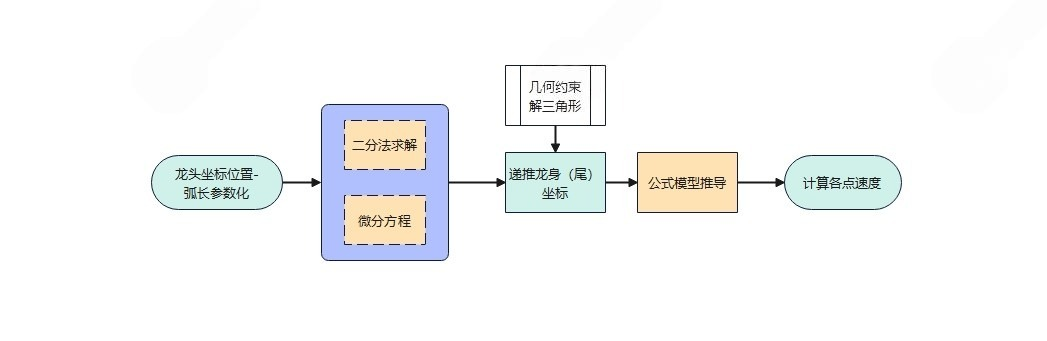
\includegraphics[width=1.3\columnwidth]{images/问题一流程图.jpeg}
    \end{adjustbox}
    \caption{问题一流程图}
    \label{fig:first}
\end{figure}

\subsection{弧长参数化和弧长函数}

由阿基米德螺线描述：
\begin{equation}
    r(\theta) = a + b\theta
\end{equation}
其中 $\theta$ 为极角，$r$ 为极径。螺距 $p=0.55\,\mathrm{m}$ 对应极角每增加 $2\pi$ 时极径的增量，同时由题图，$a$=0，故有：
\begin{equation}
    r(\theta) = b\theta
\end{equation}

\begin{equation}
b = \frac{p}{2\pi} = \frac{0.55}{2\pi}
\end{equation}
由此，螺线上任意点的直角坐标即为：
\begin{equation}
P(\theta) = (r(\theta)\cos\theta,\, r(\theta)\sin\theta)
\end{equation}
为描述龙头沿螺线的运动，需建立极角变化与弧长变化之间的关系。由上述参数方程求导，结合螺线极坐标表达式可得：
\begin{equation}
\frac{ds}{d\theta} = \sqrt{r^2 + b^2} = \sqrt{(a+b\theta)^2 + b^2}
\end{equation}
已知龙头速度恒定为$1~\text{m/s}$，经计算：
\begin{equation}
s(\theta) = \int_{\theta_0}^{\theta} \sqrt{(a+bu)^2 + b^2}\, du
\end{equation}
于是对于每一个时刻$t$,求解：
\begin{equation}
s(\theta(t)) = s(\theta_0) + t
\end{equation}
这实际上是一个一维非线性方程求根问题。



\subsection{龙头位置求解}
对于某一个具体时刻 $t = t_k$，我们要求：
\begin{equation}
f(\theta) = S(\theta) - t_k = 0
\end{equation}
由于 $S(\theta)$ 在龙头运动范围内具有单调性，因此上述方程具有唯一解。对于给定时刻 $t$，采用二分法求解 $\theta_1(t)$。
具体而言，首先确定包含根的区间 $[\theta_L,\theta_R]$，使得
\begin{equation}
f(\theta_L)f(\theta_R)<0,
\end{equation}
其中
\begin{equation}
f(\theta)=S(\theta)-t.
\end{equation}

随后取区间中点
\begin{equation}
\theta_M=\frac{\theta_L+\theta_R}{2},
\end{equation}
根据 $f(\theta_M)$ 的符号判断根所在区间，并不断缩小搜索区间。当满足
\begin{equation}
|\theta_R-\theta_L|<\varepsilon
\end{equation}
时停止迭代，并取
\begin{equation}
\theta_1(t)\approx \frac{\theta_L+\theta_R}{2}.
\end{equation}

本文取足够小的 $\varepsilon$ 以保证计算精度。求得 $\theta_1(t)$ 后，将其代入螺线参数方程，即可得到龙头前把手的位置
\begin{equation}
\boxed{
\begin{cases}
x_1(t)=(a+b\theta_1)\cos\theta_1,\\[6pt]
y_1(t)=(a+b\theta_1)\sin\theta_1.
\end{cases}
}
\end{equation}



\begin{figure}[H]
    \centering
    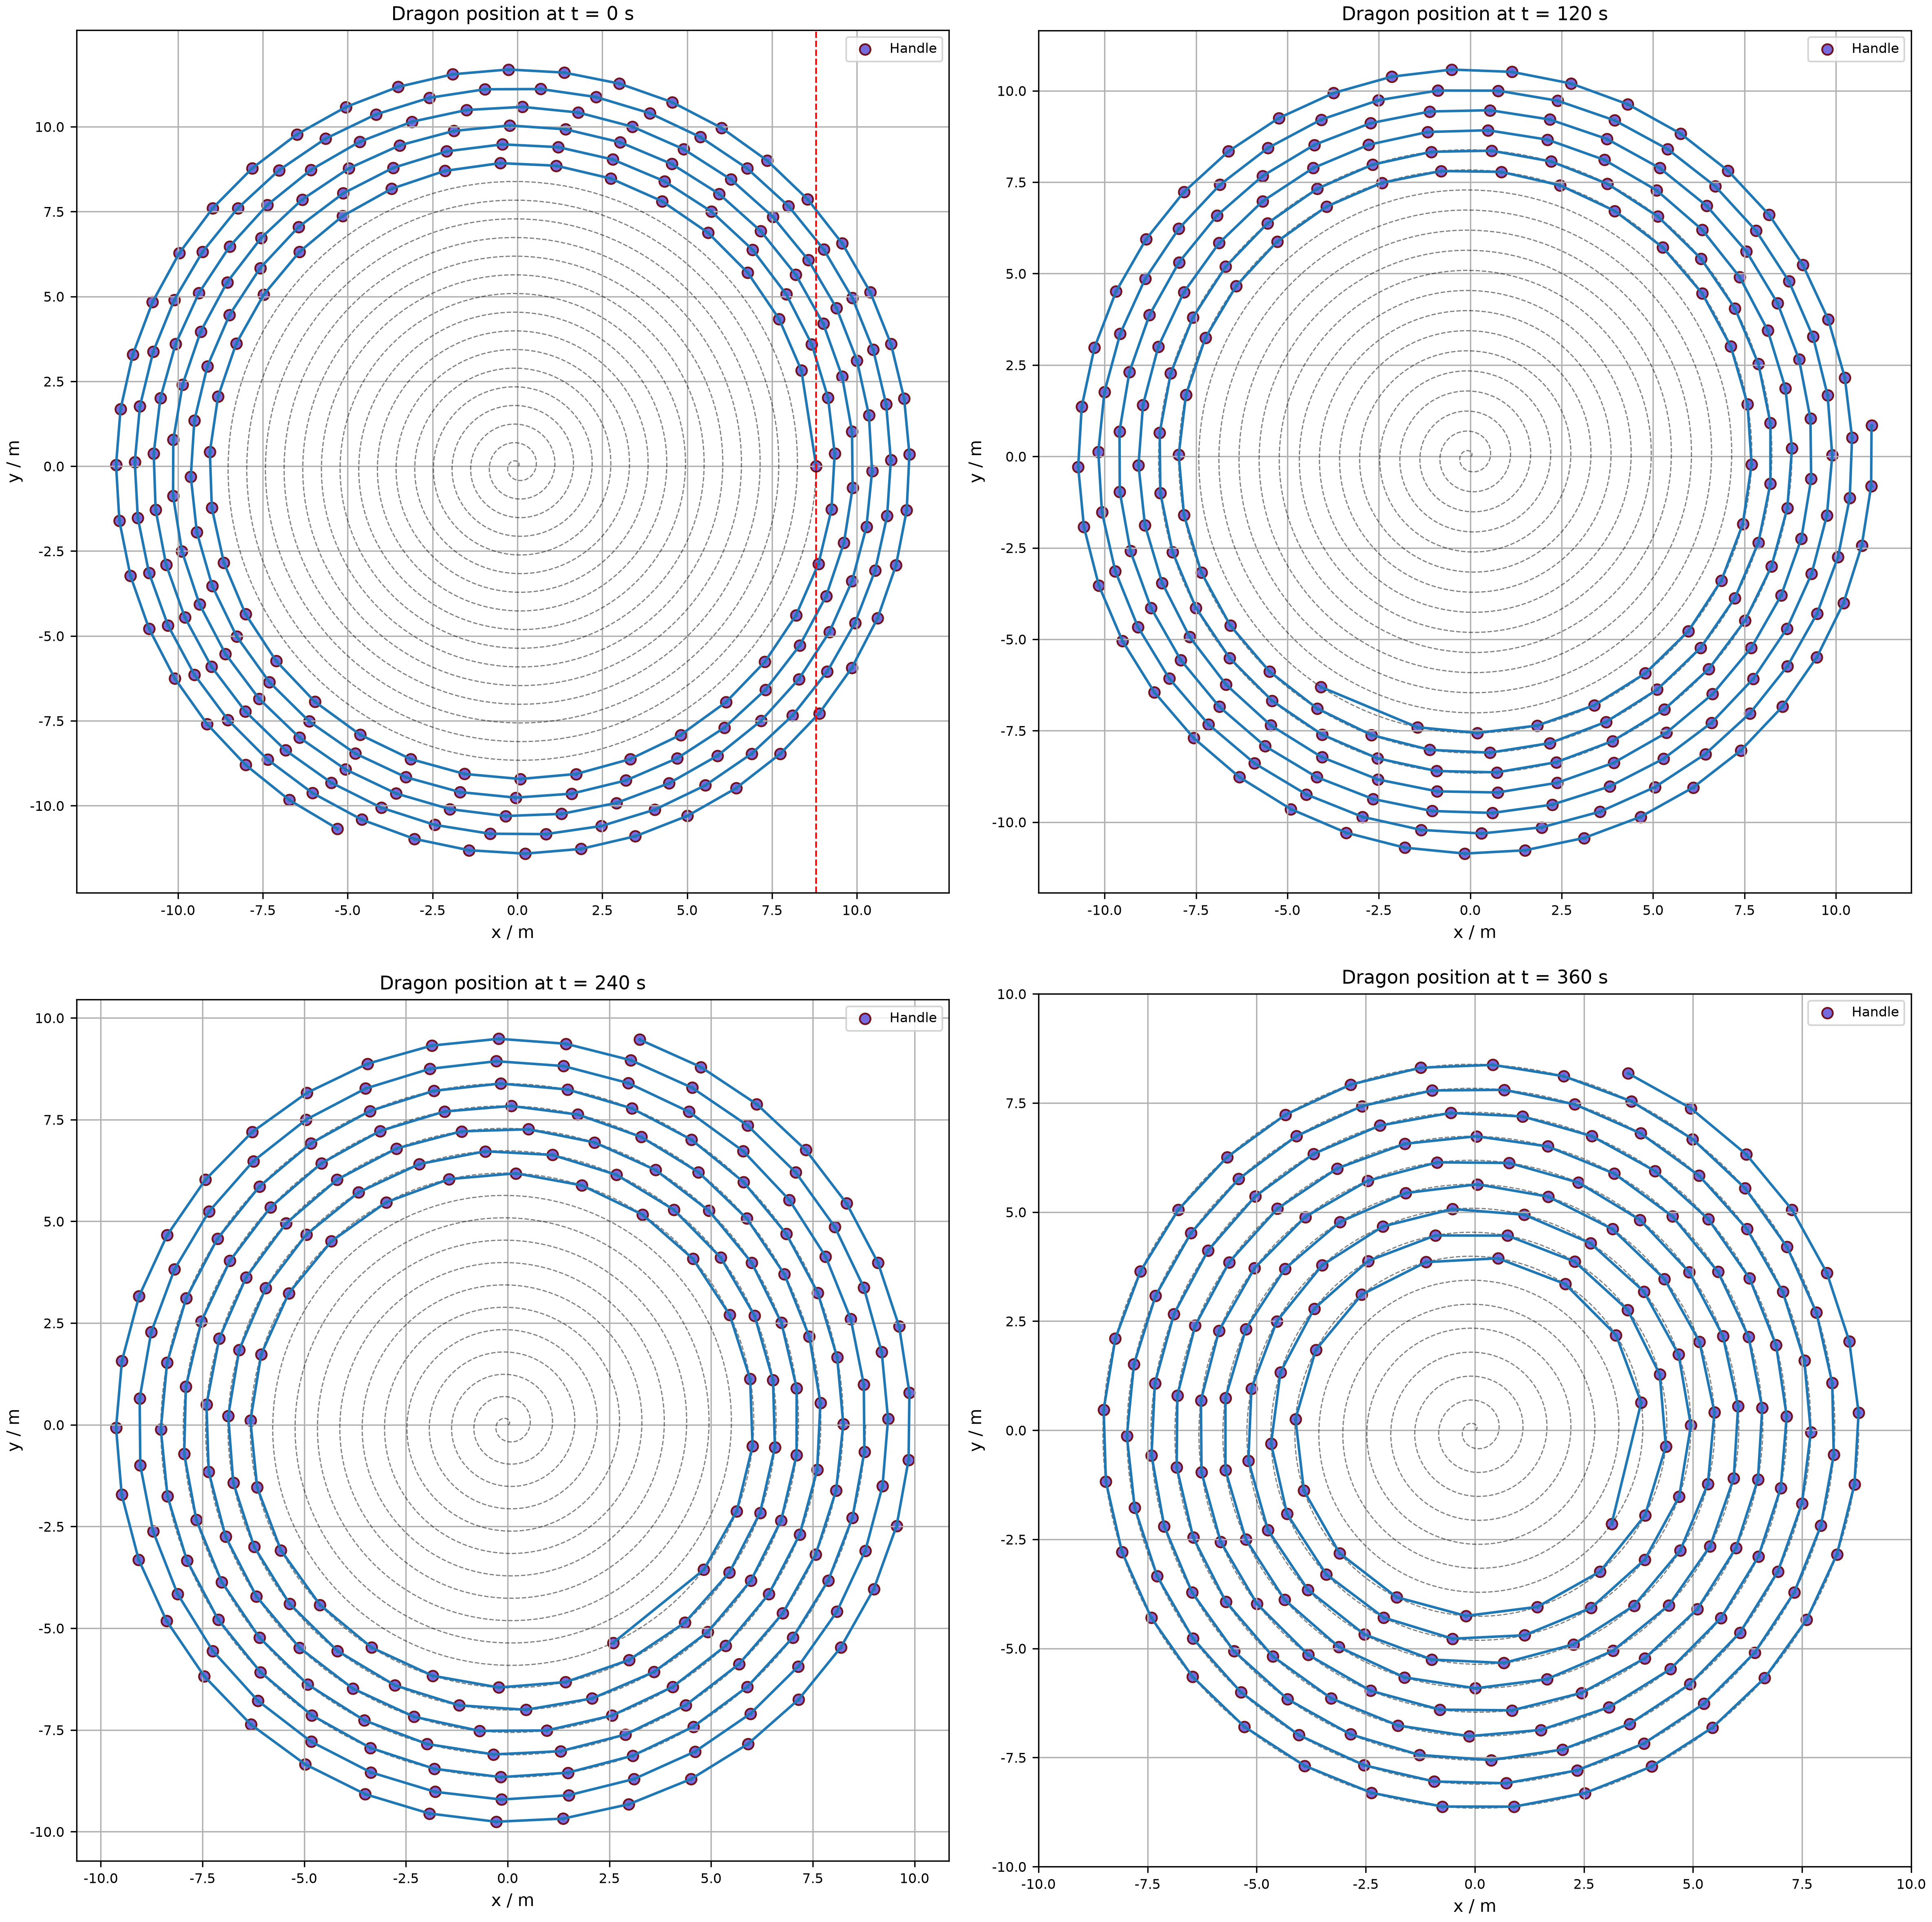
\includegraphics[width=\columnwidth]{images/螺线图 四张.png}
    \caption{板凳龙位置示意图}
    \label{fig:second}
\end{figure}

\subsection{其余把手位置求解}
对于后续其余所有把手的位置，我们仍可以采用二分检验的思想进行求解。为了充分利用几何位置关系，并减轻计算量，我们在极坐标系中的求解过程引入余弦定理进行相邻把手距离的求解。

对于任意一个把手位置：
\begin{equation}
r_i = b\theta_i
\end{equation}
设第$i$个把手和下一个相邻的把手位置的极角差值为$\Delta\theta_i$，则由距离约束：
\begin{equation}
r_{i+1} = b(\theta_i - \Delta\theta_i)
\end{equation}
根据余弦定理：
\begin{equation}
f_i(\Delta\theta_i) = r_i^2 + r_{i+1}^2 - 2r_ir_{i+1}\cos\Delta\theta_i - d_i^2 = 0
\end{equation}
这实际上是得到关于 $\Delta\theta_i$的一个一元非线性方程。
值得注意的是，这里的$d_i$并非固定值。龙头处$d_i$的值为$286$,其余情况均为$165$。

因此，在已知第 $i$个把手参数 $\theta_i$ 的情况下，只需求解上述方程即可得到 $\Delta\theta_i$，进而计算第 $i+1$ 个把手的位置。
值得注意的是，从板凳龙运动过程来看，上述方程并非任意数学根均满足实际要求，第$i+1$个把手应当：

1. 位于当前把手的盘入方向；

2. 与当前把手保持固定距离 $d_i$；

3. 在螺线上与当前把手相邻。

因此我们选取满足约束条件的最小正根作为相邻把手对应的参数间隔
\begin{equation}
\Delta\theta_i = \min\{\Delta\theta > 0 : f_i(\Delta\theta) = 0\}
\end{equation}
方程(16) 难以直接求得解析解，因此采用与 $5.2$ 节相同的二分法进行数值求根，计算精度及终止条件保持一致。
由于当
\begin{equation}
\Delta\theta = 0
\end{equation}
时相邻两个把手重合，有
\begin{equation}
f_i(0) = -d_i^2 < 0.
\end{equation}

随后从 $\Delta\theta = 0$ 开始向右搜索，确定使
\begin{equation}
f_i(\Delta\theta_R) > 0
\end{equation}
的第一个位置，从而得到满足
\begin{equation}
f_i(0)f_i(\Delta\theta_R) < 0
\end{equation}
的初始求根区间
\begin{equation}
[0,\,\Delta\theta_R].
\end{equation}

在此基础上，按照 5.2 节所述二分法不断缩小区间，最终得到
\begin{equation}
\Delta\theta_i \approx \frac{\Delta\theta_L + \Delta\theta_R}{2}.
\end{equation}

再由螺线参数方程得到其平面坐标：
\begin{equation}
\begin{cases}
x_{i+1} = b\theta_{i+1}\cos\theta_{i+1},\\[6pt]
y_{i+1} = b\theta_{i+1}\sin\theta_{i+1}.
\end{cases}
\end{equation}

将 $\theta_{i+1}$ 作为下一次递推的已知量，重复上述过程，即可依次得到
\begin{equation}
\theta_1 \rightarrow \theta_2 \rightarrow \cdots \rightarrow \theta_N
\end{equation}
从而确定该时刻舞龙队所有把手的位置。

% ==================== 表1：位置数据 ====================
\begin{table}[htbp]
    \centering
    \small  % 缩小字体以适应页面宽度
    \caption{各部位在不同时间点的位置坐标}
    \label{tab:position}
    \begin{tabular}{l|r|r|r|r|r|r}
        \hline
        时间点 & 0 s & 60 s & 120 s & 180 s & 240 s & 300 s \\
        \hline
        龙头 x (m)  & 8.800000  & 5.799209  & -4.084887 & -2.963609 & 2.594494  & 4.420274 \\
        龙头 y (m)  & 0.000000  & -5.771092 & -6.304479 & 6.094780  & -5.356743 & 2.320429 \\
        第1节龙身 x (m) & 8.363824  & 7.456758  & -1.445473 & -5.237118 & 4.821221  & 2.459489 \\
        第1节龙身 y (m) & 2.826544  & -3.440399 & -7.405883 & 4.359627  & -3.561949 & 4.402476 \\
        第51节龙身 x (m) & -9.518732 & -8.686317 & -5.543150 & 2.890455  & 5.980011  & -6.301346 \\
        第51节龙身 y (m) & 1.341137  & 2.540108  & 6.377946  & 7.249289  & -3.827758 & 0.465829 \\
        第101节龙身 x (m) & 2.913983  & 5.687116  & 5.361939  & 1.898794  & -4.917371 & -6.237722 \\
        第101节龙身 y (m) & -9.918311 & -8.001384 & -7.557638 & -8.471614 & -6.379874 & 3.936008 \\
        第151节龙身 x (m) & 10.861726 & 6.682311  & 2.388757  & 1.005154  & 2.965378  & 7.040740 \\
        第151节龙身 y (m) & 1.828753  & 8.134544  & 9.727411  & 9.424751  & 8.399721  & 4.393013 \\
        第201节龙身 x (m) & 4.555102  & -6.619664 & -10.627211 & -9.287720 & -7.457151 & -7.458662 \\
        第201节龙身 y (m) & 10.725118 & 9.025570  & 1.359847  & -4.246673 & -6.180726 & -5.263384 \\
        龙尾（后） x (m)  & -5.305444 & 7.364557  & 10.974348 & 7.383896  & 3.241051  & 1.785033 \\
        龙尾（后） y (m)  & -10.676584 & -8.797992 & 0.843473  & 7.492370  & 9.469336  & 9.301164 \\
        \hline
    \end{tabular}
\end{table}



\subsection{速度模型}

设第 $i$ 个把手的位置为
\begin{equation}
    \mathbf{r}_i=\mathbf{r}(\theta_i),
\end{equation}
相邻把手间的刚性连接长度为 $L_i$，则位置约束为
\begin{equation}
    \|\mathbf{r}_{i+1}-\mathbf{r}_i\|^2=L_i^2.
\end{equation}

对其关于时间求导，由于刚性连接长度始终不变，得到：
\begin{equation}
    (\mathbf{r}_{i+1}-\mathbf{r}_i)
    \cdot
    (\mathbf{v}_{i+1}-\mathbf{v}_i)=0.
\end{equation}

又由链式法则，
\begin{equation}
\mathbf{v}_i = \frac{d\mathbf{r}_i}{dt} = \mathbf{r}'(\theta_i)\dot\theta_i.
\end{equation}

令
\begin{equation}
    \mathbf{d}_i=\mathbf{r}_{i+1}-\mathbf{r}_i,
    \qquad
    \mathbf{T}_i=\mathbf{r}'(\theta_i),
\end{equation}
则相邻把手的角速度满足
\begin{equation}
    \dot{\theta}_{i+1}
    =
    \frac{\mathbf{d}_i\cdot\mathbf{T}_i}
    {\mathbf{d}_i\cdot\mathbf{T}_{i+1}}
    \dot{\theta}_i.
\end{equation}

龙头速度 $v_{\mathrm{head}}$ 已知，因此
\begin{equation}
    \dot{\theta}_1
    =
    -\frac{v_{\mathrm{head}}}
    {\|\mathbf{T}_1\|}.
\end{equation}

对于阿基米德螺线 $r=a+b\theta$，有
\begin{equation}
    \mathbf{T}(\theta)
    =
    \begin{pmatrix}
        b\cos\theta-r\sin\theta\\
        b\sin\theta+r\cos\theta
    \end{pmatrix},
    \qquad
    \|\mathbf{T}(\theta)\|=\sqrt{r^2+b^2}.
\end{equation}

因此
\begin{equation}
    \dot{\theta}_1
    =
    -\frac{v_{\mathrm{head}}}
    {\sqrt{r_1^2+b^2}}.
\end{equation}

最终其线速度为
\begin{equation}
    v_i
    =
    \sqrt{r_i^2+b^2}\,|\dot{\theta}_i|.
\end{equation}
由此逐节递推得到所有把手的角速度。

% ==================== 表2：速度数据 ====================
\begin{table}[htbp]
    \centering
    \small
    \caption{各部位在不同时间点的速度}
    \label{tab:speed}
    \begin{tabular}{l|r|r|r|r|r|r}
        \hline
        时间点 & 0 s & 60 s & 120 s & 180 s & 240 s & 300 s \\
        \hline
        龙头 (m/s)       & 1.000000 & 1.000000 & 1.000000 & 1.000000 & 1.000000 & 1.000000 \\
        第1节龙身 (m/s)  & 0.999971 & 0.999961 & 0.999945 & 0.999917 & 0.999859 & 0.999709 \\
        第51节龙身 (m/s) & 0.999742 & 0.999662 & 0.999538 & 0.999331 & 0.998941 & 0.998065 \\
        第101节龙身 (m/s)& 0.999575 & 0.999453 & 0.999269 & 0.998971 & 0.998435 & 0.997302 \\
        第151节龙身 (m/s)& 0.999448 & 0.999299 & 0.999078 & 0.998727 & 0.998115 & 0.996861 \\
        第201节龙身 (m/s)& 0.999348 & 0.999180 & 0.998935 & 0.998551 & 0.997894 & 0.996574 \\
        龙尾（后） (m/s) & 0.999311 & 0.999136 & 0.998883 & 0.998489 & 0.997816 & 0.996478 \\
        \hline
    \end{tabular}
\end{table}

